% =====================================================================
%  QuickPOS - Super Shop POS System
%  CSE 3206 (Software Engineering Sessional) - Lab 2
%  Project Design Report  ->  compiled to docs/Requirement_Report.pdf
%
%  Compile:  pdflatex Project_Design_Report.tex   (run twice for the TOC)
%  NOTE: all text is rendered with embedded Type 1 fonts (Latin Modern)
%        in a deliberately dark ink colour.  An earlier build of this
%        report fell back to 1-bit bitmap fonts, which produced very
%        faint, low-contrast body text; the font setup below fixes that.
% =====================================================================
\documentclass[11pt,a4paper]{article}

% ---------- page geometry ----------
\usepackage[
  top=2.35cm, bottom=2.30cm, left=2.30cm, right=2.30cm,
  headheight=15pt, headsep=0.55cm, footskip=1.05cm
]{geometry}

% ---------- fonts (Type 1, embedded - no bitmap fallback) ----------
\usepackage[T1]{fontenc}
\usepackage[utf8]{inputenc}
\usepackage{lmodern}          % Latin Modern: real Type 1 outlines
\usepackage[scaled=0.90]{helvet} % Helvetica for headings / UI chrome
\usepackage{microtype}
\usepackage{textcomp}

% ---------- colour palette (dark, high contrast) ----------
\usepackage{xcolor}
% NOTE: colortbl is deliberately NOT loaded. The colortbl build shipped with
% this TeX distribution breaks tabularx, so table headers are typeset as bold
% navy text between booktabs rules instead of as a filled colour band.
\definecolor{ink}{HTML}{111111}      % body text - near black
\definecolor{navy}{HTML}{10395E}     % section headings, table headers
\definecolor{deepteal}{HTML}{0B4F4A} % accent
\definecolor{rulegray}{HTML}{44546A} % rules and borders
\definecolor{rowalt}{HTML}{E9EFF5}   % zebra shading
\definecolor{boxbg}{HTML}{F2F5F8}   % callout background
\definecolor{boxedge}{HTML}{7A8CA0} % callout border
\definecolor{codefg}{HTML}{1B2A38}
\definecolor{gitred}{HTML}{8A1C1C}
\definecolor{gitgrn}{HTML}{14532D}

% ---------- structure ----------
\usepackage{titlesec}
\usepackage{enumitem}
\usepackage{booktabs}
\usepackage{tabularx}
\usepackage{array}
\usepackage{multirow}
\usepackage{longtable}
\usepackage{caption}
\usepackage{float}
\usepackage{needspace}
\usepackage{ragged2e}
\usepackage{listings}
\usepackage[most]{tcolorbox}
\usepackage{fancyhdr}
\usepackage[hidelinks]{hyperref}

% ---------- tikz ----------
\usepackage{tikz}
\usetikzlibrary{positioning,shapes.geometric,calc,fit,backgrounds}

% =====================================================================
%  Global appearance
% =====================================================================
\color{ink}                       % every glyph is near-black by default
\pagestyle{fancy}
\fancyhf{}
\renewcommand{\headrulewidth}{0.4pt}
\renewcommand{\footrulewidth}{0pt}
\fancyhead[L]{\footnotesize\sffamily\color{navy} QuickPOS --- Project Design Report}
\fancyhead[R]{\footnotesize\sffamily\color{navy} CSE 3206 --- Lab 2}
\fancyfoot[C]{\footnotesize\sffamily\color{rulegray}\thepage}

\titleformat{\section}
  {\needspace{4\baselineskip}\Large\sffamily\bfseries\color{navy}}
  {\thesection}{0.7em}{}[\vspace{-0.55em}\rule{\linewidth}{0.9pt}]
\titlespacing*{\section}{0pt}{1.55em}{0.85em}

\titleformat{\subsection}
  {\needspace{3\baselineskip}\large\sffamily\bfseries\color{deepteal}}
  {\thesubsection}{0.6em}{}
\titlespacing*{\subsection}{0pt}{1.05em}{0.45em}

\titleformat{\subsubsection}
  {\needspace{3\baselineskip}\normalsize\sffamily\bfseries\color{navy}}
  {\thesubsubsection}{0.6em}{}
\titlespacing*{\subsubsection}{0pt}{0.8em}{0.3em}

\setlist[itemize]{leftmargin=1.35em,itemsep=2.2pt,topsep=3pt,parsep=0pt}
\setlist[enumerate]{leftmargin=1.6em,itemsep=2.2pt,topsep=3pt,parsep=0pt}

\captionsetup{font=small,labelfont={sf,bf,color=navy},
              textfont={color=ink},skip=5pt,justification=centering}

\renewcommand{\arraystretch}{1.18}
\setlength{\tabcolsep}{5pt}

% ---- callout box ---------------------------------------------------
\newtcolorbox{notebox}[1][]{%
  colback=boxbg, colframe=boxedge, boxrule=0.6pt, arc=1.6pt,
  left=7pt, right=7pt, top=5pt, bottom=5pt, fontupper=\small,
  title={#1}, coltitle=white, colbacktitle=navy, fonttitle=\sffamily\bfseries\small
}

% ---- code / tree / git listings -----------------------------------
\definecolor{codebg}{HTML}{F4F6F8}
\definecolor{codeedge}{HTML}{B8C2CC}
\lstdefinestyle{reportstyle}{
  basicstyle=\ttfamily\footnotesize\color{codefg},
  backgroundcolor=\color{codebg},
  frame=single, rulecolor=\color{codeedge}, framerule=0.5pt,
  framesep=5pt, xleftmargin=2pt, xrightmargin=2pt,
  breaklines=true, breakatwhitespace=false,
  columns=fullflexible, keepspaces=true,
  showstringspaces=false, aboveskip=6pt, belowskip=4pt
}
\lstset{style=reportstyle}

% ---- inline code ---------------------------------------------------
\newcommand{\code}[1]{\texttt{\small\color{codefg}\detokenize{#1}}}
\newcommand{\filep}[1]{\texttt{\small\color{navy}\detokenize{#1}}}
\newcommand{\repo}{\href{https://github.com/TanzirulIslam22/QuickPOS}%
  {\texttt{\small\color{deepteal}https://github.com/TanzirulIslam22/QuickPOS}}}

% ---- user-story / acceptance-criteria helper -----------------------
\newcommand{\storytitle}[2]{%
  \par\medskip\noindent
  \textbf{\sffamily #1}\quad{\color{deepteal}\textbf{#2}}\par\nobreak\vspace{2pt}}
\newenvironment{acceptance}{%
  \begin{quote}\small\color{ink}\textbf{Acceptance criteria:}\begin{itemize}%
    \setlength{\itemsep}{1pt}\setlength{\topsep}{2pt}}{\end{itemize}\end{quote}}

% =====================================================================
\begin{document}
\color{ink}
\thispagestyle{empty}

% =====================================================================
%  COVER PAGE
% =====================================================================
\begin{center}
{\sffamily\bfseries\large\color{navy} Rajshahi University of Engineering \& Technology}\\[2pt]
{\sffamily\color{rulegray} Rajshahi---6204, Bangladesh}\\[1pt]
{\sffamily\color{rulegray} Department of Computer Science \& Engineering}\\[10pt]
\rule{\textwidth}{1.1pt}\\[-6pt]
\rule{\textwidth}{0.4pt}
\end{center}

\vspace{0.6cm}

\begin{center}
{\sffamily\bfseries\LARGE\color{navy} Project Design Report}\\[6pt]
{\sffamily\large\color{deepteal} CSE 3206 --- Software Engineering Sessional}\\[3pt]
{\sffamily\normalsize\color{ink} Lab 2: Software Process Models, Requirement Analysis \& MVP Development}\\[8pt]
{\footnotesize\sffamily\color{rulegray} Course Outcome (CO2): Design and implement software solutions that
effectively address user requirements and enhance system reliability and performance.}\\
{\footnotesize\sffamily\color{rulegray} Program Outcome (PO3): Design and Development of Software Solutions}
\end{center}

\vspace{0.5cm}

\begin{center}
\begin{minipage}{0.9\textwidth}
\centering
{\sffamily\bfseries\Huge\color{navy} QuickPOS}\\[4pt]
{\sffamily\Large\color{ink} A Super Shop Point of Sale (POS) System}\\[4pt]
{\sffamily\color{deepteal}\bfseries Minimum Viable Product (MVP) --- Increment 4 of 4}\\[10pt]
\begin{notebox}[Selected Software Process Model]
\centering\sffamily\bfseries
\textbf{Incremental Development}\\[2pt]
{\normalfont\small The system is delivered as a sequence of small, independently
demonstrable increments, each merged into \filep{main} through a reviewed pull request.}
\end{notebox}
\end{minipage}
\end{center}

\vspace{0.55cm}

\begin{center}
\renewcommand{\arraystretch}{1.35}
\begin{tabularx}{0.92\textwidth}{@{}>{\sffamily\bfseries\color{navy}}p{0.30\textwidth}X@{}}
\hline
%% no filled header band (colortbl not used)
\multicolumn{2}{c}{\sffamily\bfseries\color{navy} Submission Details}\\
\hline
Group & Group \#08 --- Section A (2nd 30)\\
\hline
Submitted by & Tanzirul Islam \textbullet{} Shuvo (Mia Shuvo) \textbullet{} Ruan (Mahdi Hosen Ruan)\\
\hline
Submitted to & Course Teacher, Department of Computer Science \& Engineering, RUET\\
\hline
GitHub repository & \repo\\
\hline
Project Design Report & \filep{docs/Requirement_Report.pdf} (source: \filep{docs/Project_Design_Report.tex})\\
\hline
Date of submission & 01 October 2026\\
\hline
\end{tabularx}
\end{center}

\vfill
\begin{center}
\footnotesize\sffamily\color{rulegray}
Lab 2 deliverables: GitHub repository (branches, pull requests, commit history) \textbullet{}
Project Design Report \textbullet{} MVP demonstration \textbullet{} Individual viva
\end{center}

\clearpage

% =====================================================================
%  TABLE OF CONTENTS
% =====================================================================
{\sffamily\bfseries\large\color{navy}Table of Contents}\par
\vspace{4pt}\hrule\vspace{10pt}
\tableofcontents
\vspace{10pt}\hrule
\clearpage

% =====================================================================
\section{Team Information and Work Ownership}
% =====================================================================
\addcontentsline{toc}{section}{Team Information and Work Ownership}

This section is the single authoritative record of \emph{who contributed which part of
the system}. It is reproduced in the repository (\filep{README.md} and
\filep{docs/TEAM_WORKFLOW.md}) so that the contribution split can be verified against
the Git commit history rather than taken on trust.

\subsection{Team members, roles and branches}

\begin{table}[H]
\centering\footnotesize
\setlength{\tabcolsep}{3pt}
\begin{tabularx}{\textwidth}{@{}>{\bfseries\sffamily\color{navy}}p{0.10\textwidth}>{\raggedright\arraybackslash}p{0.27\textwidth}>{\raggedright\arraybackslash}p{0.11\textwidth}>{\raggedright\arraybackslash}p{0.23\textwidth}>{\raggedright\arraybackslash}X@{}}
\toprule
\multicolumn{5}{c}{\sffamily\bfseries\color{navy} Table: Member, Git identity, feature branch and module responsibility}\\[2pt]
\midrule
Team Member & GitHub Author / Committed As & Role & Git Branch & Module Responsibility\\
\hline
Tanzirul Islam & \code{TanzirulIslam22} \newline \code{tanzirul.islam56@gmail.com} & Team Lead \& Backend / Core Developer & \filep{tanzirul/mvp-base}\newline\filep{tanzirul/report-lab2} & Repository and GitHub workflow setup; Express server, MongoDB models and REST routes; React application shell and session gate; Login, Products and POS pages; cash handling and stock deduction; sales history; report and documentation\\
Shuvo & \code{Hi-There-shuvo} \newline \code{saddamshuvo1710@gmail.com} & Frontend Feature Developer & \filep{shuvo/category-receipt} & Printable invoice / receipt module (\filep{Invoice.jsx}) and its integration into the checkout success path in \filep{POS.jsx}, including the print stylesheet\\
Ruan & \code{mahdi-ruan} \newline \code{mhr359359@gmail.com} & Frontend Feature Developer & \filep{ruan/dashboard} & Planned sales summary dashboard increment (PR \#2); delivered increment contains route-level hardening of \filep{saleRoutes.js}; outstanding summary widget carried to the backlog as B-01\\
\bottomrule
\end{tabularx}
\end{table}

\subsection{Ownership map}

Figure~\ref{fig:ownership} maps each member to the part of the system that member owns.
The same mapping is applied file by file in the module breakdown of Section~\ref{sec:mvp}.

\begin{figure}[H]
\centering
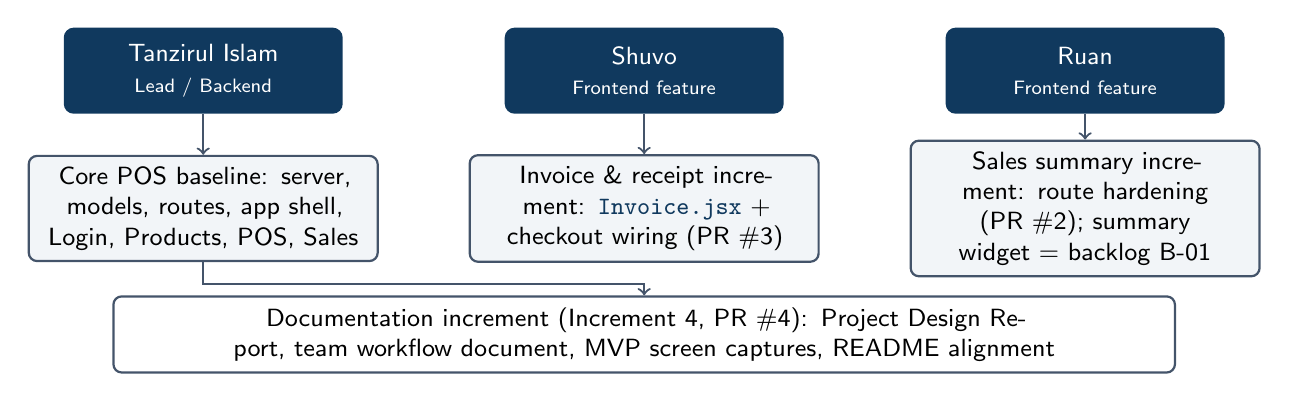
\begin{tikzpicture}[
  font=\sffamily\small,
  member/.style={draw=navy, very thick, rounded corners=3pt, fill=navy,
                 text=white, align=center, inner sep=5pt, minimum width=3.5cm, minimum height=1.05cm},
  part/.style={draw=rulegray, thick, rounded corners=3pt, fill=boxbg, align=center,
               inner sep=4pt, minimum height=0.72cm, text width=4.15cm},
  link/.style={->, rulegray, thick}
]
  \node[member] (t) at (-5.6,0) {Tanzirul Islam\\\scriptsize Lead / Backend};
  \node[member] (s) at ( 0.0,0) {Shuvo\\\scriptsize Frontend feature};
  \node[member] (r) at ( 5.6,0) {Ruan\\\scriptsize Frontend feature};

  \node[part] (t1) at (-5.6,-1.75) {Core POS baseline: server, models, routes, app shell, Login, Products, POS, Sales};
  \node[part] (s1) at ( 0.0,-1.75) {Invoice \& receipt increment: \filep{Invoice.jsx} + checkout wiring (PR \#3)};
  \node[part] (r1) at ( 5.6,-1.75) {Sales summary increment: route hardening (PR \#2); summary widget = backlog B-01};

  \node[part, fill=white, text width=13.2cm] (t2) at (0,-3.35)
        {Documentation increment (Increment 4, PR \#4): Project Design Report, team workflow document, MVP screen captures, README alignment};

  \draw[link] (t) -- (t1);
  \draw[link] (s) -- (s1);
  \draw[link] (r) -- (r1);
  \draw[link] (t1.south) -- ++(0,-0.28) -| (t2.north);
\end{tikzpicture}
\caption{Work ownership: member $\rightarrow$ feature branch $\rightarrow$ module.}
\label{fig:ownership}
\end{figure}

\subsection{Collaboration rules followed by the team}

\begin{itemize}
  \item \filep{main} is the only integration branch; no member pushes directly to it.
  \item Every increment is developed on its own \code{member/feature} branch, committed with a
        meaningful message, pushed, and submitted as a pull request against \filep{main}.
  \item A pull request is reviewed by at least one other member before it is merged.
  \item Each pull request states, in its description, which requirements it satisfies and
        which requirements remain open. Where an increment is closed with work still
        outstanding, the gap is recorded as a numbered backlog item instead of being left
        implicit (see Section~\ref{sec:mvp-backlog}).
\end{itemize}

% =====================================================================
\section{Project Title and Overview}
% =====================================================================
\addcontentsline{toc}{section}{Project Title and Overview}

\begin{center}
{\sffamily\bfseries\Large\color{navy} QuickPOS --- A Super Shop Point of Sale (POS) System}
\end{center}

QuickPOS is a web-based billing and stock system for a small neighbourhood super shop. It
replaces the shop's paper bills and stock notebooks with a single screen on which a cashier
logs in, builds a bill, takes the customer's cash, and is told exactly how much change to
return --- while every sale is written to a database and the stock count of each sold item is
reduced automatically.

QuickPOS is this lab's Minimum Viable Product (MVP): a small but complete and functional
slice of a larger system. It deliberately contains only what is needed to demonstrate that
the core billing concept is technically feasible --- authentication, one core domain (the
product-and-sale domain), basic persistence and a simple user interface --- and nothing
else. The code is written as a set of small, replaceable modules so that the following labs
of the semester (design patterns, testing) can build on it without a rewrite.

% =====================================================================
\section{Problem Statement}
% =====================================================================

A single-bay super shop in Bangladesh typically records its sales on paper bills kept in a
box, and tracks remaining stock in a separate notebook. The result is four recurring,
concrete problems:

\begin{itemize}
  \item \textbf{Slow and error-prone billing.} Every sale requires the cashier to look up a
        price in the notebook and write the bill by hand. At peak hours a queue forms, and
        arithmetic mistakes in the total or in the change are common.
  \item \textbf{No trustworthy stock count.} Because the notebook is updated by hand and only
        at the shop owner's discretion, the recorded stock routinely disagrees with the
        shelf. The owner then either sells an item that is not there, or discards items that
        were actually available.
  \item \textbf{No record of cash movement.} Change given to a customer is calculated
        mentally. When the drawer does not balance at the end of the day there is no way to
        determine which bill was miscalculated, so daily takings cannot be verified.
  \item \textbf{No sales history for decisions.} Because bills are paper, the owner cannot
        answer simple questions such as which product sells most, what the daily revenue was,
        or which items need restocking.
\end{itemize}

QuickPOS addresses each of these directly: an itemised billing screen that computes the
total, an explicit cash-handling panel that computes and validates change before a sale can
be committed, automatic stock deduction that refuses a sale exceeding available stock, and a
persistent sales history that can be reviewed at any time.

% =====================================================================
\section{Project Objectives}
% =====================================================================

\begin{enumerate}
  \item Provide a fast, single-screen billing interface that a new cashier can operate
        without training.
  \item Maintain accurate product information --- name, price, stock and category --- in one
        place, with the catalogue maintained through the application itself.
  \item Compute the bill total automatically from the cart so that no arithmetic is done by
        hand at the counter.
  \item Record the cash actually received from the customer, compute the change to return,
        and \emph{reject} the sale whenever the cash received is less than the total.
  \item Reduce product stock automatically as part of the checkout transaction, and refuse
        any sale that would drive stock below zero.
  \item Persist every completed sale --- its items, total, cash paid, change and timestamp ---
        and display the recent sales history.
  \item Produce a printable invoice for each sale so the customer leaves with a receipt.
  \item Gate the whole system behind a staff login so that the billing screen is not open to
        walk-in customers.
  \item Ship demonstrable sample data so that the MVP can be reviewed immediately after
        installation, without manual database preparation.
  \item Demonstrate a functioning Incremental Development process executed by a
        three-member team through feature branches and reviewed pull requests.
\end{enumerate}

% =====================================================================
\section{Stakeholder Analysis}
% =====================================================================

\begin{table}[H]
\centering\small
\begin{tabularx}{\textwidth}{@{}>{\bfseries\sffamily\color{navy}}p{0.16\textwidth}p{0.36\textwidth}X@{}}
\toprule
\multicolumn{3}{c}{\sffamily\bfseries\color{navy} Table: Stakeholder, interest or need, and primary interactions with the system}\\[2pt]
\midrule
Stakeholder & Interest / Need & Primary Interactions\\
\hline
Shop Owner & Daily revenue figures, control over the product catalogue and stock levels, and a low-cost tool that does not need an IT background to operate & Reviews the sales history; adds, edits and removes products; monitors stock after every checkout\\
Cashier & A fast billing screen that is easy to learn, that never lets an incorrect total reach the customer, and that always states the change to return & Logs in, builds a cart, enters the cash received, completes the checkout, prints the invoice\\
Customer & An accurate total, the correct change, and a receipt as proof of purchase & Interacts indirectly: is served by the cashier's billing screen; receives the printed invoice\\
System Administrator & Control of the product data and of who may use the system & Manages products, resets the session, seeds demonstration data\\
Regulator / Auditor (indirect) & Traceability of individual sales transactions & Would consume the persisted sale records (date, items, total, cash paid, change) exported from the sales history\\
\bottomrule
\end{tabularx}
\end{table}

All stakeholders identified above expect the system to be fast, reliable and simple to use.
These three expectations are the origin of most of the non-functional requirements in
Section~\ref{sec:nfr}.

% =====================================================================
\section{Scope of the Project}
% =====================================================================

\subsection{In scope for this lab}

\begin{itemize}
  \item Staff authentication and session handling for a single shop terminal.
  \item Product catalogue with list, add and delete operations.
  \item Billing: cart with quantities, automatic total, cash-entered payment, change
        calculation and a printable invoice.
  \item Automatic stock validation and deduction at checkout.
  \item Persistent sales history.
  \item Demonstration (seed) data.
\end{itemize}

\subsection{Explicitly out of scope for the MVP}

Supplier and purchase records, bar-code scanning, multi-branch stock transfer, customer
loyalty accounts, employee salary calculation, taxation, hardware receipt printers, offline
mode, and internet-facing deployment. Recording what is \emph{not} being built is part of
keeping an MVP an MVP; the excluded items are carried in the backlog of
Section~\ref{sec:mvp-backlog} for later increments.

% =====================================================================
\section{Functional Requirements}
% =====================================================================
\label{sec:fr}

The requirements below are traceable to the delivered code. The \emph{Implemented in}
column states where each requirement is satisfied and which team member's increment
delivered it. Requirements FR-01 to FR-18 are the MVP requirement set; FR-06 is available at
the API level and is queued for the user interface in backlog item B-02.

\begin{longtable}{@{}p{0.09\textwidth}p{0.055\textwidth}p{0.47\textwidth}p{0.30\textwidth}@{}}
\caption{Functional requirements with implementation traceability.}\label{tab:fr}\\
\toprule
%% no filled header band (colortbl not used)
\multicolumn{4}{c}{\sffamily\bfseries\color{navy} Table: Functional requirements and where each is implemented}\\
\midrule
\endfirsthead
\toprule
%% no filled header band (colortbl not used)
\multicolumn{4}{c}{\sffamily\bfseries\color{navy} Functional requirements (continued)}\\
\midrule
\endhead
\bottomrule
\endfoot
\textbf{ID} & \textbf{Status} & \textbf{Requirement} & \textbf{Implemented in}\\
\hline
FR-01 & Done & The system shall authenticate a staff member with a username and a password before any billing screen is shown. & \filep{Login.jsx}; credential pair \code{admin / 1234}\\
FR-02 & Done & The system shall keep the authenticated session across page reloads and shall end it on logout, returning the user to the login screen. & \filep{App.jsx} via \code{localStorage}\\
FR-03 & Done & The system shall list every product with its name, unit price and current stock level. & \filep{POS.jsx}, \filep{Products.jsx}; \code{GET /api/products}\\
FR-04 & Done & The system shall allow a new product to be added with name, price and stock. & \filep{Products.jsx}; \code{POST /api/products}\\
FR-05 & Done & The system shall allow an existing product to be deleted. & \filep{Products.jsx}; \code{DELETE /api/products/:id}\\
FR-06 & API only & The system shall allow an existing product's details to be updated. & \code{PUT /api/products/:id} implemented in \filep{productRoutes.js}; no user interface yet (backlog B-02)\\
FR-07 & Done & The system shall allow a product to be added to the bill, and repeated additions of the same product shall increase its quantity. & \filep{POS.jsx} \code{add()} function\\
FR-08 & Done & The system shall allow the cashier to empty the current bill without starting a session again. & \filep{POS.jsx} \emph{Clear} button\\
FR-09 & Done & The system shall compute the running bill total from the cart contents. & \filep{POS.jsx} \code{total} reducer\\
FR-10 & Done & The system shall accept the amount of cash handed over by the customer. & \filep{POS.jsx} \code{paidAmount} input, shown once the cart is non-empty\\
FR-11 & Done & The system shall compute the change to return as (cash received $-$ bill total) and display it live while the cashier types. & \filep{POS.jsx} \code{change} value and \emph{Change to Return} panel\\
FR-12 & Done & The system shall refuse to complete a sale when the cash received is less than the bill total, both in the user interface and on the server. & \filep{POS.jsx} disables \emph{Checkout}; \filep{saleRoutes.js} returns HTTP 400\\
FR-13 & Done & On a successful sale the system shall reduce the stock of every sold item by the quantity sold. & \filep{saleRoutes.js} \code{p.stock -= it.qty}\\
FR-14 & Done & The system shall refuse a sale for any item whose requested quantity exceeds the available stock. & \filep{saleRoutes.js} stock check before any write\\
FR-15 & Done & The system shall store every completed sale with its itemised lines, total, cash received, change and timestamp. & \filep{Sale.js} model; \code{POST /api/sales}\\
FR-16 & Done & The system shall display the most recent sales, newest first, with each bill's total, cash paid and change. & \filep{Sales.jsx}; \code{GET /api/sales} (latest 50)\\
FR-17 & Done & After a successful sale the system shall present a printable invoice listing every line, the subtotal, the cash received, the change returned and the grand total. & \filep{Invoice.jsx}; \code{window.print()} with an \code{@media print} stylesheet\\
FR-18 & Done & The system shall be able to populate the catalogue with demonstration products so the MVP can be demonstrated immediately. & \filep{server.js} \code{GET /api/seed}\\
\end{longtable}

% =====================================================================
\section{Non-Functional Requirements}
% =====================================================================
\label{sec:nfr}

\begin{longtable}{@{}p{0.09\textwidth}p{0.20\textwidth}p{0.62\textwidth}@{}}
\caption{Non-functional requirements.}\label{tab:nfr}\\
\toprule
%% no filled header band (colortbl not used)
\multicolumn{3}{c}{\sffamily\bfseries\color{navy} Table: Non-functional requirements}\\
\midrule
\endfirsthead
\toprule
%% no filled header band (colortbl not used)
\multicolumn{3}{c}{\sffamily\bfseries\color{navy} Non-functional requirements (continued)}\\
\midrule
\endhead
\bottomrule
\endfoot
\textbf{ID} & \textbf{Category} & \textbf{Requirement}\\
\hline
NFR-01 & Performance & A checkout transaction shall complete within 2 seconds on the shop's local network, excluding the cashier's typing time.\\
NFR-02 & Performance & Re-opening the product list after a sale shall not require a full page reload; the billing screen shall refresh its stock view after each checkout.\\
NFR-03 & Usability & The complete billing task shall be performable from a single screen using only the keyboard and one pointing device, with no training manual and no multi-page wizard.\\
NFR-04 & Usability & Destructive and irreversible actions (completing a sale, clearing a bill) shall be visually distinguishable from routine actions.\\
NFR-05 & Availability & The system shall run on a single computer inside the shop and shall continue to work with no internet connection.\\
NFR-06 & Portability & The system shall run on any operating system through a current desktop web browser, with no platform-specific component.\\
NFR-07 & Maintainability & Source shall be separated into a frontend module, a backend module, a route layer and a data-model layer; each page and each route shall be independently replaceable.\\
NFR-08 & Maintainability & All backend calls from the frontend shall pass through one helper module so that the endpoint contract is defined in exactly one place.\\
NFR-09 & Security & No billing, catalogue or sales screen shall be reachable without an authenticated session.\\
NFR-10 & Security / Integrity & Payment validation shall be repeated on the server; the client-side check shall be treated as a usability aid only, never as the enforcement point.\\
NFR-11 & Reliability & A sale shall be written to the database before the billing screen is cleared, so that an interrupted session cannot lose a completed transaction.\\
NFR-12 & Data Integrity & Stock shall never be recorded as negative; a sale exceeding available stock shall be rejected as a whole, without partially applying it.\\
NFR-13 & Scalability & The product catalogue shall remain operable at 10\,000 product records without a change in the interaction model.\\
NFR-14 & Traceability & Each sale shall record its timestamp so that the day's takings can be reconstructed after the fact.\\
NFR-15 & Printability & The invoice shall have a dedicated print stylesheet so that on-screen controls (buttons, backdrop) do not appear on the printed receipt.\\
\end{longtable}

% =====================================================================
\section{User Stories and Use Cases}
% =====================================================================

Six user stories are given below, each with an acceptance criterion written in
Given/When/Then form. The acceptance criteria are the definition of ``done'' for the
increment that delivers the story.

\storytitle{US-1}{Staff authentication (Cashier)}
As a cashier, I want to log in with my staff credentials so that the billing screen is not
open to any customer or visitor.

\begin{acceptance}
  \item \textbf{Given} the application is opened with no active session, \textbf{when} the
        cashier submits \code{admin / 1234}, \textbf{then} the billing screen is shown and
        the session survives a page reload.
  \item \textbf{Given} the application is opened with no active session, \textbf{when} any
        other credential pair is submitted, \textbf{then} the login screen remains and no
        billing data is displayed.
  \item \textbf{Given} an active session, \textbf{when} \emph{Logout} is pressed,
        \textbf{then} the session is destroyed and the login screen is shown again.
\end{acceptance}

\storytitle{US-2}{Building a bill (Cashier)}
As a cashier, I want to add products to a bill and see the running total so that I can serve
a customer quickly without doing arithmetic myself.

\begin{acceptance}
  \item \textbf{Given} the billing screen, \textbf{when} the cashier presses \emph{Add} on a
        product, \textbf{then} that product appears in the bill with quantity 1 and the total
        increases by the unit price.
  \item \textbf{Given} a product is already in the bill, \textbf{when} \emph{Add} is pressed
        again, \textbf{then} only its quantity increases and no duplicate line is created.
  \item \textbf{Given} a bill with three lines, \textbf{when} the cashier inspects the
        header, \textbf{then} the displayed total equals the sum of price $\times$ quantity
        over all three lines.
\end{acceptance}

\storytitle{US-3}{Cash handling and change (Cashier)}
As a cashier, I want to type in the cash the customer handed over and be shown the change, so
that I return the correct amount and never have to calculate it mentally.

\begin{acceptance}
  \item \textbf{Given} a bill of 490 Tk, \textbf{when} the cashier enters 500 Tk,
        \textbf{then} the panel shows \emph{Change to Return: 10 Tk} and the \emph{Checkout}
        button becomes enabled.
  \item \textbf{Given} a bill of 490 Tk, \textbf{when} the cashier enters 400 Tk,
        \textbf{then} the panel marks the amount as \emph{insufficient}, the \emph{Checkout}
        button stays disabled, and no sale is created.
  \item \textbf{Given} an enabled \emph{Checkout} button, \textbf{when} it is pressed,
        \textbf{then} the API rejects the request with HTTP 400 if, and only if, the server
        also computes the payment as insufficient.
\end{acceptance}

\storytitle{US-4}{Automatic stock control (Shop Owner)}
As a shop owner, I want the stock of an item to fall automatically when it is sold, so that
the system never sells something the shelf does not have.

\begin{acceptance}
  \item \textbf{Given} an item with 100 units in stock, \textbf{when} a bill of 2 units is
        completed, \textbf{then} the stored stock becomes 98.
  \item \textbf{Given} an item with 1 unit in stock, \textbf{when} a bill of 5 units is
        submitted, \textbf{then} the whole sale is rejected and the stored stock is left
        unchanged at 1.
\end{acceptance}

\storytitle{US-5}{Printable invoice (Cashier \& Customer)}
As a cashier, I want a printable invoice to appear automatically after a sale so that the
customer receives a receipt and I have proof of the transaction.

\begin{acceptance}
  \item \textbf{Given} a completed checkout, \textbf{when} the invoice appears,
        \textbf{then} it lists every sold line with quantity, unit price and line amount,
        plus the subtotal, the cash received, the change returned and the grand total.
  \item \textbf{Given} the invoice is on screen, \textbf{when} \emph{Print Invoice} is
        pressed, \textbf{then} the browser print dialog opens and the printed page contains
        the receipt only --- no buttons and no dimmed backdrop.
\end{acceptance}

\storytitle{US-6}{Sales history (Shop Owner)}
As a shop owner, I want to see previous bills with their total, cash paid and change, so
that I can check the day's takings.

\begin{acceptance}
  \item \textbf{Given} at least one completed sale, \textbf{when} the \emph{Sales} screen is
        opened, \textbf{then} the bills are listed newest first, each with its timestamp,
        itemised lines, total, cash paid and change.
  \item \textbf{Given} no sale has been recorded, \textbf{when} the \emph{Sales} screen is
        opened, \textbf{then} an explicit \emph{No sales yet} message is shown instead of an
        empty page.
\end{acceptance}

% =====================================================================
\section{Assumptions and Constraints}
% =====================================================================

\subsection{Assumptions}

\begin{itemize}
  \item The shop operates a single billing terminal, so there is no requirement for
        concurrent cashiers or multi-session stock locking.
  \item All staff are trusted employees of one shop, so a single shared staff account is
        acceptable for the MVP; differentiated roles are deferred (backlog B-06).
  \item Prices do not change during an open bill, so the price captured at checkout is the
        authoritative price for that sale.
  \item The shop can run a small always-on computer with Node.js and a local MongoDB
        instance; cloud hosting is not required.
  \item Electrical power and network stability inside the shop are the shop's existing
        responsibility.
\end{itemize}

\subsection{Constraints}

\begin{itemize}
  \item \textbf{Time.} The project is a single laboratory session of the first milestone of
        a semester-long project, developed by a three-member student team.
  \item \textbf{Scope.} The lab explicitly requires a Minimum Viable Product only; feature
        count is not the measure of success, engineering method is.
  \item \textbf{Process.} Every member must contribute through Git using a feature branch and
        a pull request; direct pushes to \filep{main} are not permitted by the team's own
        working agreement.
  \item \textbf{Future labs.} The code must remain modular, because later labs will add
        design patterns and automated tests on top of this codebase.
  \item \textbf{Tooling.} Only freely available, quickly learnable technology may be used
        within the time available, which excludes heavyweight enterprise frameworks.
\end{itemize}

% =====================================================================
\section{Selected Software Process Model: Incremental Development}
% =====================================================================
\label{sec:model}

The team selected the \textbf{Incremental Development} process model. QuickPOS is delivered
as a sequence of increments. Each increment adds a coherent slice of functionality to a
system that is already running, and each increment is integrated into the main branch
through a reviewed pull request, so that at the end of every increment there is a
\emph{working, demonstrable} product rather than a partial one.

This choice also matches the process model suggested for this project in the lab
assignment (\emph{Super Shop POS System} $\rightarrow$ \emph{Incremental}), but the selection
below is justified on the project's own characteristics rather than on the suggestion alone
(Section~\ref{sec:justification}).

\subsection{How the model is applied}

\begin{itemize}
  \item \textbf{Requirements are decomposed, not frozen.} The requirement set of
        Section~\ref{sec:fr} is partitioned into increments that each deliver an end-to-end
        slice --- for example ``cart $\rightarrow$ total $\rightarrow$ cash $\rightarrow$
        change'' is one slice, not four separate features.
  \item \textbf{Each increment is integrated.} Work happens on a feature branch and reaches
        \filep{main} only through a reviewed pull request, so the main branch always holds a
        working system.
  \item \textbf{Each increment is verified and demonstrated.} An increment is closed only
        after it has been run end-to-end and shown to the team.
  \item \textbf{Unfinished work is carried, not hidden.} When an increment is closed with
        scope outstanding, the gap is recorded as a numbered backlog item and planned into a
        later increment.
\end{itemize}

\subsection{Increment plan and delivery record}

Table~\ref{tab:increments} is the increment plan and, at the same time, the record of what
was actually delivered.

\setlength{\tabcolsep}{3pt}%
\begin{longtable}{@{}p{0.07\textwidth}p{0.19\textwidth}p{0.24\textwidth}p{0.245\textwidth}p{0.07\textwidth}p{0.115\textwidth}@{}}
\caption{Increment plan and delivery record.}\label{tab:increments}\\
\toprule
%% no filled header band (colortbl not used)
\multicolumn{6}{c}{\sffamily\bfseries\color{navy} Table: Increments, branches, pull requests and outcome}\\
\midrule
\endfirsthead
\toprule
%% no filled header band (colortbl not used)
\multicolumn{6}{c}{\sffamily\bfseries\color{navy} Increments (continued)}\\
\midrule
\endhead
\bottomrule
\endfoot
\textbf{Inc.} & \textbf{Focus} & \textbf{Delivered functionality} & \textbf{Branch / PR} & \textbf{Owner} & \textbf{Outcome}\\
\hline
1 & POS core baseline & Authenticated application shell and tab navigation; login/logout; product catalogue (list, add, delete); cart with quantities and automatic total; Express server with MongoDB \code{Product} and \code{Sale} models; full REST route layer; demonstration seed endpoint; sales history; README and the GitHub workflow & \filep{tanzirul/mvp-base} (direct commit) & Tanzirul Islam & Delivered\\
2 & Sales summary & Planned increment: an aggregated sales-summary endpoint and a summary dashboard page showing total and today's revenue & \filep{ruan/dashboard}, PR \#2 & Ruan & Partially delivered\\
3 & Invoice \& receipt & Printable invoice module with itemised lines, subtotal, cash paid, change, grand total, and a dedicated \code{@media print} stylesheet; wired into the checkout success path in place of a browser alert & \filep{shuvo/category-receipt}, PR \#3 & Shuvo & Delivered\\
4 & Report \& collaboration hardening & This Project Design Report; \filep{docs/TEAM_WORKFLOW.md}; MVP screen captures; README aligned with the delivered system; report build corrected to embed outline fonts instead of bitmap fonts & \filep{tanzirul/report-lab2}, PR \#4 & Tanzirul Islam & Delivered\\
\end{longtable}

\subsection{Honest statement of Increment 2}
\label{sec:increment2}

Increment 2 is reported as partially delivered rather than as complete. Pull request \#2
was opened with the message ``add sales summary and endpoint and dashboard page'', but the
merged diff contains only route-level changes in \filep{saleRoutes.js} and a comment
cleanup in \filep{App.jsx}; neither a summary endpoint nor a dashboard page reached
\filep{main}. Rather than reporting the increment as complete, the team records the
outstanding summary widget as backlog item B-01 in Section~\ref{sec:mvp-backlog} and
schedules it for the next increment. Reporting this gap is the point of using an
incremental model: an unfinished increment has a visible, nameable remainder, and the
remainder does not block the delivery of the other three increments.

\subsection{Figure: incremental delivery for QuickPOS}

\begin{figure}[H]
\centering
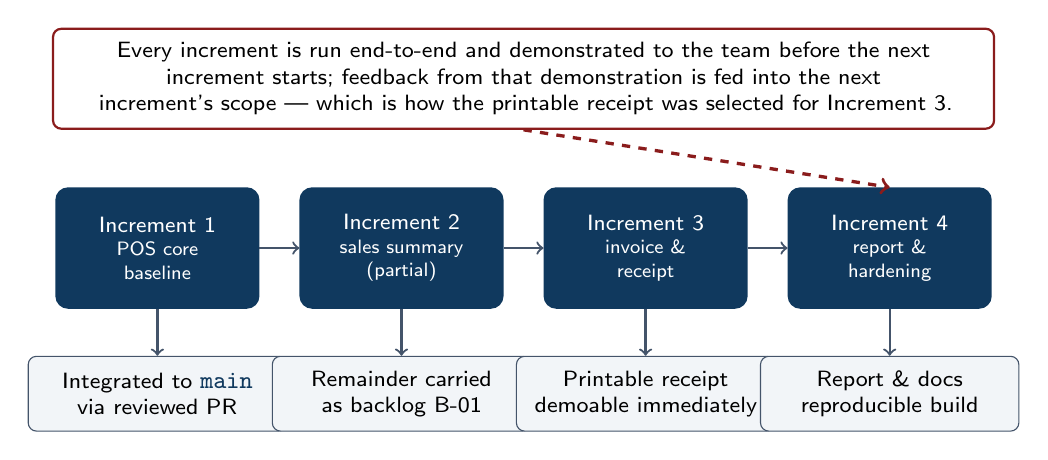
\begin{tikzpicture}[
  font=\sffamily\footnotesize,
  inc/.style={draw=navy, very thick, fill=navy, text=white, rounded corners=4pt,
              minimum width=2.55cm, minimum height=1.5cm, align=center, inner sep=3pt},
  note/.style={draw=rulegray, rounded corners=3pt, fill=boxbg, align=center,
               inner sep=4pt, minimum height=0.95cm, text width=3.0cm},
  link/.style={->, rulegray, thick},
  fb/.style={->, gitred, very thick, dashed}
]
  \node[inc] (i1) at (-4.65,0)  {Increment 1\\[-1pt]\scriptsize POS core\\[-1pt]\scriptsize baseline};
  \node[inc] (i2) at (-1.55,0) {Increment 2\\[-1pt]\scriptsize sales summary\\[-1pt]\scriptsize (partial)};
  \node[inc] (i3) at ( 1.55,0) {Increment 3\\[-1pt]\scriptsize invoice \&\\[-1pt]\scriptsize receipt};
  \node[inc] (i4) at ( 4.65,0) {Increment 4\\[-1pt]\scriptsize report \&\\[-1pt]\scriptsize hardening};

  \draw[link] (i1)--(i2);
  \draw[link] (i2)--(i3);
  \draw[link] (i3)--(i4);

  \node[note] (n1) at (-4.65,-1.85) {Integrated to \filep{main}\\via reviewed PR};
  \node[note] (n2) at (-1.55,-1.85) {Remainder carried\\as backlog B-01};
  \node[note] (n3) at ( 1.55,-1.85) {Printable receipt\\demoable immediately};
  \node[note] (n4) at ( 4.65,-1.85) {Report \& docs\\reproducible build};

  \draw[link] (i1.south)--(n1.north);
  \draw[link] (i2.south)--(n2.north);
  \draw[link] (i3.south)--(n3.north);
  \draw[link] (i4.south)--(n4.north);

  \node[draw=gitred, thick, fill=white, rounded corners=3pt, inner sep=5pt,
        align=center, text width=11.6cm] (feedback) at (0,2.15)
        {Every increment is run end-to-end and demonstrated to the team before the next\\
         increment starts; feedback from that demonstration is fed into the next\\
         increment's scope --- which is how the printable receipt was selected for Increment 3.};

  \draw[fb] (feedback.south) -- (i4.north);
\end{tikzpicture}
\caption{Incremental delivery of QuickPOS: each increment is integrated into \filep{main} through a reviewed pull request and demonstrated before the next increment begins.}
\label{fig:increments}
\end{figure}

% =====================================================================
\section{Justification of the Selected Process Model}
% =====================================================================
\label{sec:justification}

\begin{itemize}
  \item \textbf{The deliverable is defined as an MVP.} The lab asks for a small prototype that
        demonstrates feasibility, not for a complete system. Incremental development starts
        from a thin working core and grows; it does not require the complete specification to
        exist before any code is written, which is exactly the situation here.
  \item \textbf{The requirements are clear but naturally decomposable.} POS requirements are
        well understood and stable, so they can be planned up front. What makes them a good
        fit for increments is that they partition cleanly into end-to-end slices --- a cart
        without a total is not demonstrable, and a total without cash handling is not a POS
        bill. Each slice fits in one increment.
  \item \textbf{Early and continuous client feedback.} Each increment ends in something the
        course teacher can actually run. Cash handling, for example, was shown as a working
        button in Increment 1 and only then hardened, while the printable receipt --- an
        addition that was not in the original plan --- was pulled forward into Increment 3
        after the demonstration.
  \item \textbf{It maps directly onto the required GitHub workflow.} One increment, one
        feature branch, one pull request, one merge. The process model and the collaboration
        requirement reinforce each other instead of competing.
  \item \textbf{It suits a three-member parallel team.} The three module boundaries
        (baseline backend and core screens, receipt, summary) map onto three branch owners who
        can work concurrently with minimal merge contention.
  \item \textbf{It fits a semester-long project.} The lab manual states that each lab builds on
        the previous one. An incremental model keeps the backlog open across labs, so design
        patterns and testing can be added as later increments on a system that is already
        running --- no migration is needed.
  \item \textbf{Low blast radius.} If one increment is rejected or defective, only that slice
        is affected; the previously merged increments keep working. In Increment 2 this was
        demonstrated in practice: the incomplete dashboard affected nothing else.
  \item \textbf{Requirements traceability is natural.} Because every increment is small, each
        requirement can be linked to the pull request that delivered it, which is what
        Table~\ref{tab:fr} does.
\end{itemize}

% =====================================================================
\section{Comparison with Alternative Process Models}
% =====================================================================

\subsection{Comparative summary}

\begin{table}[H]
\centering\small
%% no zebra striping (colortbl not used)
\begin{tabularx}{\textwidth}{@{}>{\bfseries\sffamily\color{navy}}p{0.17\textwidth}p{0.20\textwidth}p{0.17\textwidth}p{0.17\textwidth}p{0.20\textwidth}@{}}
\toprule
%% no filled header band (colortbl not used)
\multicolumn{5}{c}{\sffamily\bfseries\color{navy} Comparison of candidate process models}\\
\midrule
Criterion & \textbf{Incremental} & Waterfall & Spiral & Scrum\\
\hline
Requirement stability needed & Medium --- stable but decomposable & High --- must be frozen before coding & Medium & Low to medium\\
Feedback frequency & Every increment & Once, at the end & Every loop & Every sprint\\
Time to first demonstrable product & End of Increment 1 (days) & End of implementation (weeks) & After the first loop & End of Sprint 1 (days)\\
Documentation overhead & Light --- increment plan \& backlog & Heavy --- full upfront specification & Heavy --- risk analysis per loop & Medium --- backlog, reviews, retrospectives\\
Change cost after delivery & Low --- isolated to the next increment & Very high --- re-work of completed phases & Medium & Low to medium\\
Fit for a 3-member team on a short lab timeline & Strong & Weak & Weak & Moderate to strong\\
\end{tabularx}
\end{table}

\subsection{Why Waterfall was less suitable}

Waterfall requires the requirement set to be frozen before design begins and delivers the
system in one pass at the end. Two properties of QuickPOS rule it out. First, the deliverable
is an MVP that must be demonstrable early, whereas Waterfall's first demonstrable output
arrives only after implementation is complete --- the opposite of what this lab asks for.
Second, the requirements were \emph{not} fully frozen in advance: the printable invoice was
not part of the initial plan and entered the project as Increment 3 after the team saw how
weak a plain browser alert was as sale confirmation. In Waterfall that addition would have
required reopening a completed design phase, which is slow and expensive for a small team.

\subsection{Why Spiral was less suitable}

Spiral is designed for projects with significant technical or business uncertainty, where
each loop performs systematic risk analysis and prototype evaluation. QuickPOS carries very
little technical risk: the hard parts (cart arithmetic, change calculation, stock
deduction) are simple transactions, and the stack --- React, Express, MongoDB --- is familiar
and well documented. Spiral's risk-analysis machinery would have consumed a disproportionate
share of a one-session lab timeline while reducing essentially none of the actual project
risk. Spiral would be appropriate for this domain if, for example, the shop required offline
first operation with later synchronisation, a genuinely uncertain hardware integration.

\subsection{Why Agile Scrum was less suitable}

Scrum delivers working software in short cycles --- the same core benefit that Incremental
provides --- but it adds role separation, sprint ceremonies, estimation in story points and
retrospectives. For a one-session academic MVP with a three-student team, stable technology
and a requirement set already documented in Section~\ref{sec:fr}, this ceremony adds process
weight without adding feedback that the team did not already have. The team adopted the parts
of Scrum that genuinely helped --- a visible increment plan, a prioritised backlog, and a
review before each merge --- and obtained the same benefit with far less overhead.

\subsection{The remaining models}

\begin{itemize}
  \item \textbf{Prototype.} Suited to projects where the user interface or the workflow is
        genuinely unknown and must be explored before it can be specified. QuickPOS's
        workflow (a POS screen has been understood for decades) does not need exploring, and
        throwing away a prototype afterwards would waste the work rather than refine it.
  \item \textbf{RAD.} Suited to large teams building business applications from detailed,
        pre-existing specifications on a fixed, compressed timeline. QuickPOS is a
        three-member team with a small requirement set, so RAD's component-based tooling
        would be disproportionate.
  \item \textbf{Agile XP.} Its emphasis on test-first development, pair programming and small
        releases is compatible with the approach, but the pair-programming discipline is not
        practical for three part-time students on different machines. Automated testing is
        planned as a later increment (backlog B-07).
  \item \textbf{Kanban.} A strong fit for continuous flow with prioritised demand, but there
        is no continuous flow to manage here: work arrives in deliberate, time-boxed
        increments per the lab schedule, which is precisely what Incremental models.
\end{itemize}

% =====================================================================
\section{MVP Design Overview}
% =====================================================================
\label{sec:mvp}

\subsection{Technology stack}

\begin{reporttable}{Technology used for the MVP}
Layer & Technology & Version / Note\\
\hline
Frontend framework & React with Vite & React 18.3, Vite 5.4 --- component-based UI with a fast development server and production build\\
Styling & Tailwind CSS & 3.4 --- utility-first styling; no separate UI framework or icon package required\\
Frontend routing & In-application page state & \filep{App.jsx} holds the active page in component state; a full router is unnecessary for three screens\\
Backend runtime & Node.js with Express & Express 4.19 --- minimal REST layer, JSON body parsing and CORS enabled\\
Database & MongoDB via Mongoose & Mongoose 8.5 --- \code{Product} and \code{Sale} collections with schema-level validation and defaults\\
Configuration & dotenv & \code{server/.env} for the database URI and port; \filep{.env} is never committed\\
Version control & Git and GitHub & Feature branches, pull requests, reviewed merges\\
Reporting & LaTeX & \filep{docs/Project_Design_Report.tex} compiled with \code{pdflatex}; outline fonts are embedded so the report stays legible on screen and in print\\
\end{reporttable}

\subsection{Architecture}

QuickPOS is a three-tier client--server application. Figure~\ref{fig:arch} shows the
request path for a checkout, which is the most demanding operation in the system because it
reads products, validates payment, writes stock changes and inserts a sale.

\begin{figure}[H]
\centering
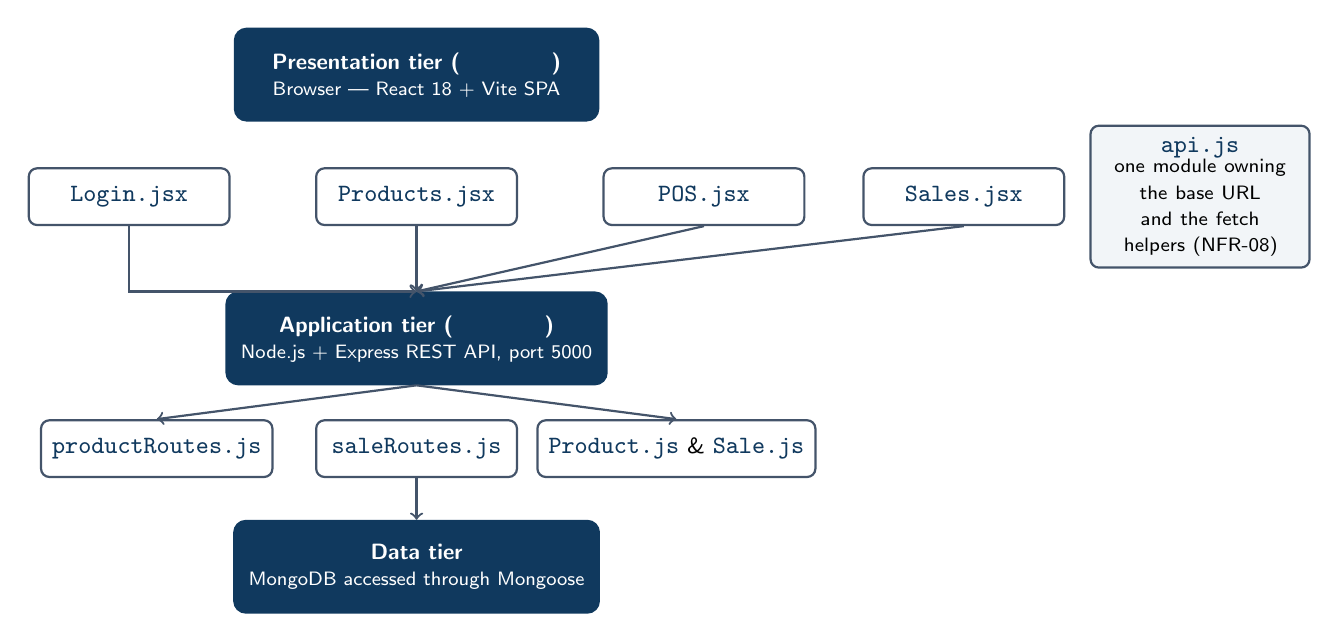
\begin{tikzpicture}[
  font=\sffamily\footnotesize,
  tier/.style={draw=navy, very thick, rounded corners=4pt, fill=navy, text=white,
               align=center, inner sep=5pt, minimum width=4.6cm, minimum height=1.15cm},
  box/.style={draw=rulegray, thick, rounded corners=3pt, fill=white, align=center,
              inner sep=4pt, minimum width=2.55cm, minimum height=0.72cm},
  link/.style={->, rulegray, thick}
]
  \node[tier] (browser) at (0,0)
        {\textbf{\color{white}Presentation tier (\filep{client/})}\\
         \scriptsize Browser --- React 18 + Vite SPA};
  \node[box] (login) at (-3.65,-1.55) {\filep{Login.jsx}};
  \node[box] (prod)  at ( 0.00,-1.55) {\filep{Products.jsx}};
  \node[box] (pos)   at ( 3.65,-1.55) {\filep{POS.jsx}};
  \node[box] (sales) at ( 6.95,-1.55) {\filep{Sales.jsx}};
  \node[box, fill=boxbg, text width=2.5cm, minimum height=0.95cm] (helper) at (9.95,-1.55)
        {\textbf{\filep{api.js}}\\[-2pt]\scriptsize one module owning the base URL and the fetch helpers (NFR-08)};

  \node[tier] (api) at (0,-3.35)
        {\textbf{\color{white}Application tier (\filep{server/})}\\
         \scriptsize Node.js + Express REST API, port 5000};
  \node[box] (pr) at (-3.30,-4.75) {\filep{productRoutes.js}};
  \node[box] (sr) at ( 0.00,-4.75) {\filep{saleRoutes.js}};
  \node[box] (md) at ( 3.30,-4.75) {\filep{Product.js} \& \filep{Sale.js}};

  \node[tier] (db) at (0,-6.25)
        {\textbf{\color{white}Data tier}\\
         \scriptsize MongoDB accessed through Mongoose};

  \draw[link] (login.south) |- (api.north);
  \draw[link] (prod.south)  -- (api.north);
  \draw[link] (pos.south)   -- (api.north);
  \draw[link] (sales.south) -- (api.north);
  \draw[link] (api.south) -- (pr.north);
  \draw[link] (api.south) -- (md.north);
  \draw[link] (sr.south) -- (db.north);
\end{tikzpicture}
\caption{Three-tier architecture of the QuickPOS MVP. The checkout path is
\filep{POS.jsx} $\rightarrow$ \filep{saleRoutes.js} $\rightarrow$ \code{Sale} and \code{Product}.}
\label{fig:arch}
\end{figure}

\subsection{Backend interface}

\begin{table}[H]
\centering\small
%% no zebra striping (colortbl not used)
\begin{tabularx}{\textwidth}{@{}p{0.10\textwidth}p{0.26\textwidth}Xp{0.22\textwidth}@{}}
\toprule
%% no filled header band (colortbl not used)
\multicolumn{4}{c}{\sffamily\bfseries\color{navy} REST endpoints exposed by the MVP}\\
\midrule
Method & Endpoint & Purpose & Used by\\
\hline
GET & \code{/api/products} & List all products, sorted by name & \filep{POS.jsx}, \filep{Products.jsx}\\
POST & \code{/api/products} & Create a product & \filep{Products.jsx}\\
PUT & \code{/api/products/:id} & Update a product & (API only --- backlog B-02)\\
DELETE & \code{/api/products/:id} & Delete a product & \filep{Products.jsx}\\
GET & \code{/api/sales} & Most recent 50 sales, newest first & \filep{Sales.jsx}\\
POST & \code{/api/sales} & Checkout: validates payment, decrements stock, stores the sale & \filep{POS.jsx}\\
GET & \code{/api/seed} & Populate the catalogue with demonstration products & Demonstration setup\\
\end{tabularx}
\end{table}

\subsection{Module breakdown and ownership}

\begin{table}[H]
\centering\small
%% no zebra striping (colortbl not used)
\begin{tabularx}{\textwidth}{@{}p{0.17\textwidth}p{0.30\textwidth}Xp{0.17\textwidth}@{}}
\toprule
%% no filled header band (colortbl not used)
\multicolumn{4}{c}{\sffamily\bfseries\color{navy} Table: Modules, files, responsibility and owner}\\
\midrule
Module & Files & Responsibility & Owner\\
\hline
Authentication & \filep{pages/Login.jsx}, \filep{App.jsx} & Credential gate, session persistence in \code{localStorage}, logout, page navigation & Tanzirul Islam\\
Product catalogue & \filep{pages/Products.jsx}, \filep{routes/productRoutes.js}, \filep{models/Product.js} & List, add and delete products; price, stock and category fields & Tanzirul Islam\\
Billing / POS & \filep{pages/POS.jsx}, \filep{routes/saleRoutes.js} & Cart with quantities, running total, checkout transaction, stock validation and deduction, sale persistence & Tanzirul Islam\\
Cash handling & \filep{pages/POS.jsx}, \filep{routes/saleRoutes.js} & Cash-received input, live change calculation, insufficient-payment rejection on both tiers & Tanzirul Islam\\
Invoice / receipt & \filep{pages/Invoice.jsx} & Printable receipt modal: itemised lines, subtotal, cash paid, change, grand total, print stylesheet, print and close actions & Shuvo\\
Sales history & \filep{pages/Sales.jsx} & Newest-first list of bills with total, cash paid and change; empty state message & Tanzirul Islam\\
Sales summary dashboard & --- (not delivered) & Planned aggregated revenue view; merged PR delivered route hardening only; remainder recorded as backlog B-01 & Ruan\\
API client helper & \filep{src/api.js} & Base URL plus \code{getJSON} / \code{postJSON}, centralising the endpoint contract & Tanzirul Islam\\
Seed data & \filep{server/server.js} & Application bootstrap, MongoDB connection, \code{/api/seed} demonstration fixtures & Tanzirul Islam\\
Documentation \& report & \filep{docs/}, \filep{README.md}, \filep{screenshots/} & Project Design Report, team workflow document, MVP screen captures, repository documentation & Tanzirul Islam\\
\end{tabularx}
\end{table}

\subsection{Component structure}

\begin{figure}[H]
\centering
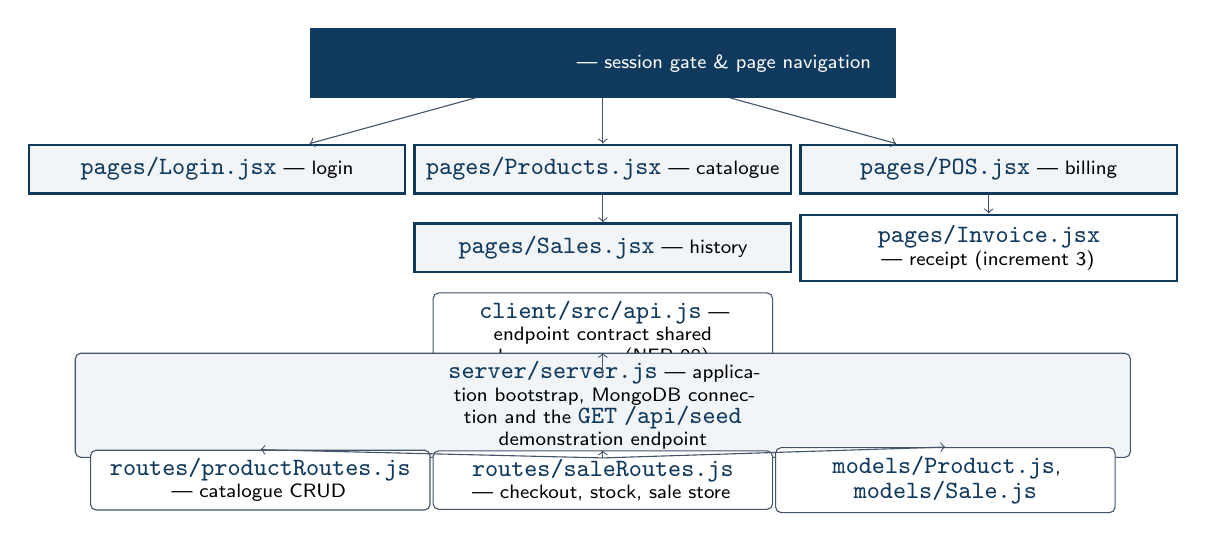
\begin{tikzpicture}[
  font=\sffamily\scriptsize,
  root/.style={draw=navy, very thick, fill=navy, text=white, align=center,
               inner sep=5pt, minimum width=7.4cm, minimum height=0.85cm},
  lvl1/.style={draw=navy, thick, fill=boxbg, align=center, inner sep=4pt,
               minimum height=0.62cm, text width=4.5cm},
  lvl2/.style={draw=rulegray, rounded corners=2pt, fill=white, align=center,
               inner sep=3pt, minimum height=0.55cm, text width=4.1cm},
  link/.style={->, rulegray}
]
  \node[root] (app) at (0,0)
        {\filep{client/src/App.jsx} --- session gate \& page navigation};
  \node[lvl1] (login) at (-4.90,-1.35) {\filep{pages/Login.jsx} --- login};
  \node[lvl1] (prod)  at ( 0.00,-1.35) {\filep{pages/Products.jsx} --- catalogue};
  \node[lvl1] (pos)   at ( 4.90,-1.35) {\filep{pages/POS.jsx} --- billing};
  \node[lvl1] (sal)   at ( 0.00,-2.35) {\filep{pages/Sales.jsx} --- history};
  \node[lvl1, fill=white] (inv) at (4.90,-2.35)
        {\filep{pages/Invoice.jsx} --- receipt (increment 3)};

  \node[lvl2, fill=white] (helper) at (0,-3.45)
        {\filep{client/src/api.js} --- endpoint contract shared by every page (NFR-08)};

  \node[lvl2, fill=boxbg, minimum width=13.4cm] (server) at (0,-4.35)
        {\filep{server/server.js} --- application bootstrap, MongoDB connection and the \filep{GET /api/seed} demonstration endpoint};
  \node[lvl2] (pr) at (-4.35,-5.30) {\filep{routes/productRoutes.js} --- catalogue CRUD};
  \node[lvl2] (sr) at ( 0.00,-5.30) {\filep{routes/saleRoutes.js} --- checkout, stock, sale store};
  \node[lvl2] (md) at ( 4.35,-5.30) {\filep{models/Product.js}, \filep{models/Sale.js}};

  \draw[link] (app) -- (login);
  \draw[link] (app) -- (prod);
  \draw[link] (app) -- (pos);
  \draw[link] (pos)  -- (inv);
  \draw[link] (prod) -- (sal);
  \draw[link] (helper.south) -- (server.north);
  \draw[link] (server.south) -- (pr.north);
  \draw[link] (server.south) -- (sr.north);
  \draw[link] (server.south) -- (md.north);
\end{tikzpicture}
\caption{Component structure of the MVP. \filep{Invoice.jsx} was added as a separate
component in Increment 3 rather than being inlined into the billing screen, which keeps the
billing logic readable and allows the print stylesheet to be scoped to one component.}
\label{fig:components}
\end{figure}

\subsection{Cash handling as a transaction}

The cash-handling rule is deliberately implemented twice, on purpose:

\begin{center}
\begin{tabular}{@{}ll@{}}
\code{total}  $=$ & $\sum$ (unit price $\times$ quantity) over all cart lines\\
\code{change} $=$ & \code{paidAmount} $-$ \code{total}\\[3pt]
accept the sale $\iff$ & \code{paidAmount} $\ge$ \code{total} \quad and \quad cart is non-empty
\end{tabular}
\end{center}

The client disables the \emph{Checkout} button and shows a live \emph{Change to Return} panel
so the cashier gets immediate feedback (FR-11, FR-12). The server repeats the same
comparison and returns HTTP 400 if it fails, before any stock is written --- the client check
is a usability aid, the server check is the enforcement point (NFR-10). The stock check
(FR-14) runs inside the same loop that builds the bill items, and because the loop
validates every line before any value is written back, a rejected sale leaves stock
completely untouched (NFR-12).

\subsection{Sale document}

\begin{table}[H]
\centering\small
%% no zebra striping (colortbl not used)
\begin{tabularx}{0.86\textwidth}{@{}p{0.20\textwidth}p{0.20\textwidth}X@{}}
\toprule
%% no filled header band (colortbl not used)
\multicolumn{3}{c}{\sffamily\bfseries\color{navy} Table: Fields of the \code{Sale} document}\\
\midrule
Field & Type & Meaning\\
\hline
\code{items} & Array of objects & The sold lines, each holding \code{productId}, \code{name}, \code{price} and \code{qty}. Name and price are copied at sale time so the bill stays historically correct even if the catalogue changes later.\\
\code{total} & Number & Bill total computed from the lines (required).\\
\code{paidAmount} & Number & Cash received from the customer; defaults to the total for exact-payment sales.\\
\code{change} & Number & Cash to return, i.e. \code{paidAmount} $-$ \code{total}.\\
\code{date} & Date & Timestamp of the transaction, defaulting to the moment of creation; drives the sales-history ordering (NFR-14).\\
\end{tabularx}
\end{table}

\subsection{MVP demonstration screens}

The following captures were taken from the running MVP. The API was populated with the
demonstration products of \code{/api/seed}.

\begin{figure}[H]
\centering
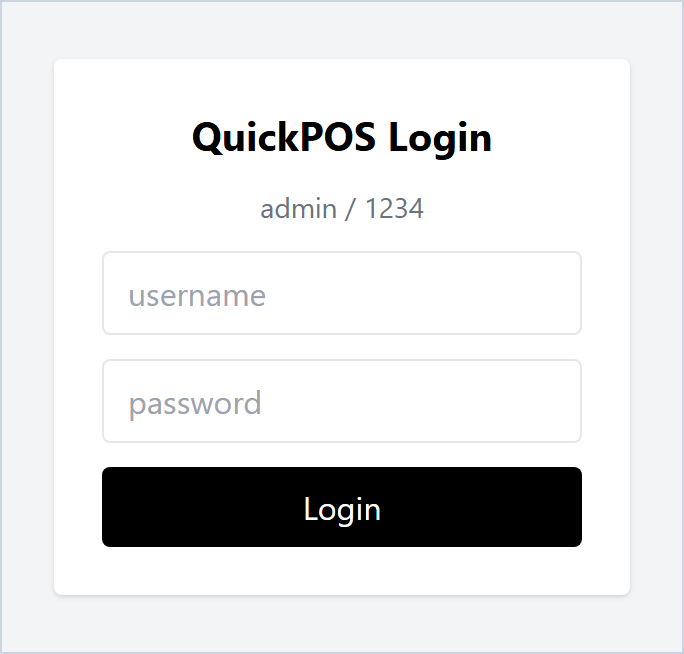
\includegraphics[width=0.30\textwidth]{../screenshots/01_login.png}
\caption{US-1 --- staff login gate. No billing screen is reachable without a session.}
\label{fig:shot-login}
\end{figure}

\begin{figure}[H]
\centering
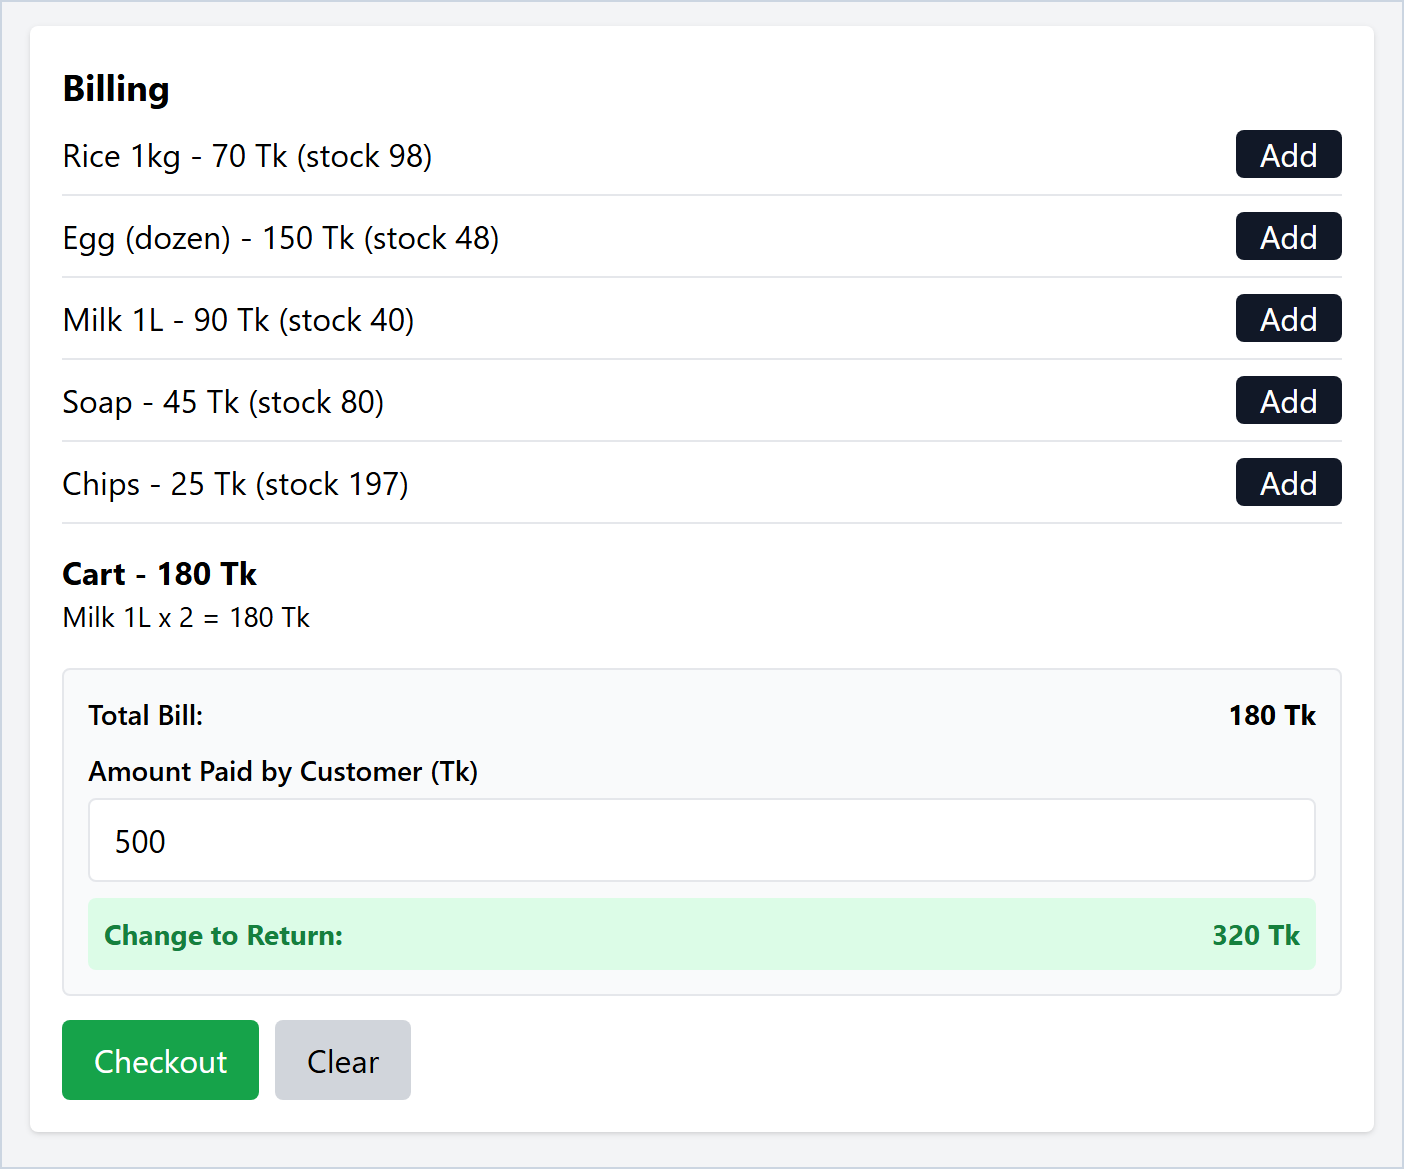
\includegraphics[width=0.62\textwidth]{../screenshots/02_billing_cart.png}
\caption{US-2 and US-3 --- billing screen with a four-line bill (490 Tk), cash received of
500 Tk entered, and the \emph{Change to Return} panel showing 10 Tk with the
\emph{Checkout} button enabled.}
\label{fig:shot-billing}
\end{figure}

\begin{figure}[H]
\centering
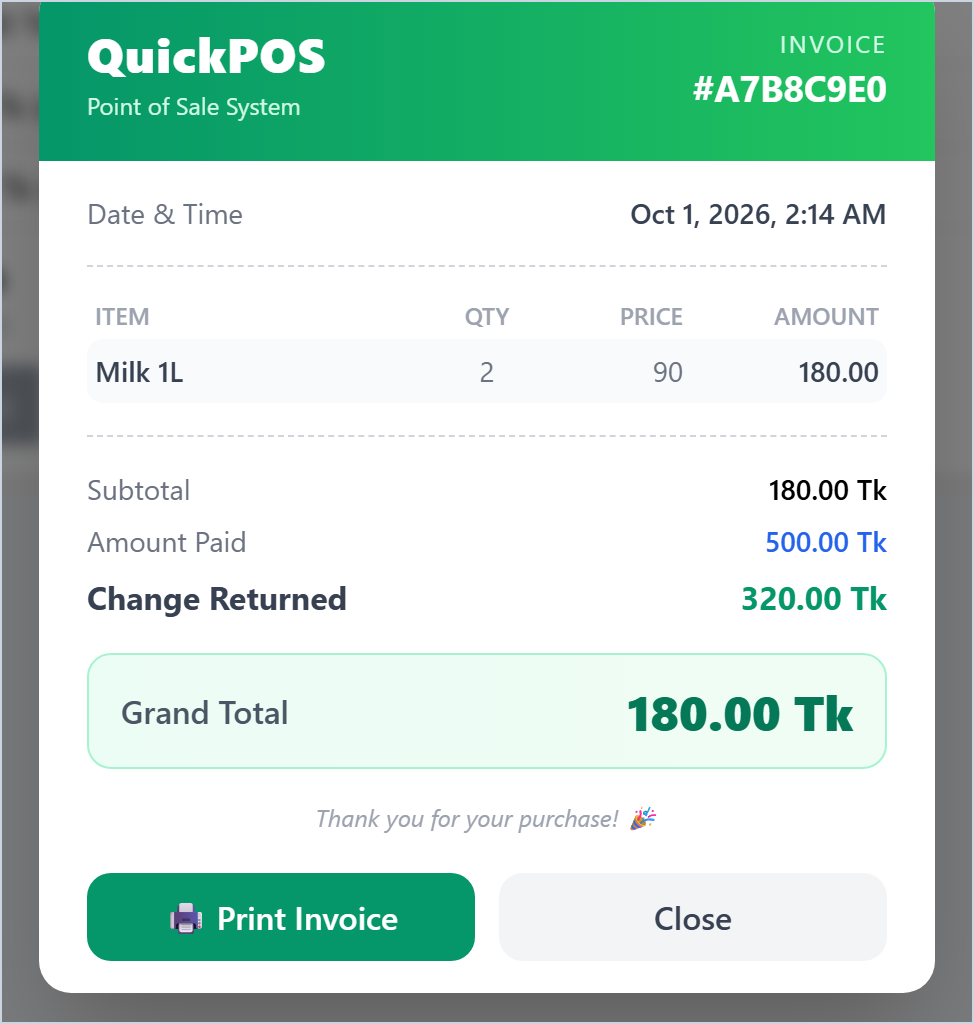
\includegraphics[width=0.44\textwidth]{../screenshots/03_invoice_receipt.png}
\caption{US-5 --- printable invoice produced by Increment 3, showing itemised lines,
subtotal 490 Tk, amount paid 500 Tk, change returned 10 Tk and the grand total.}
\label{fig:shot-invoice}
\end{figure}

\begin{figure}[H]
\centering
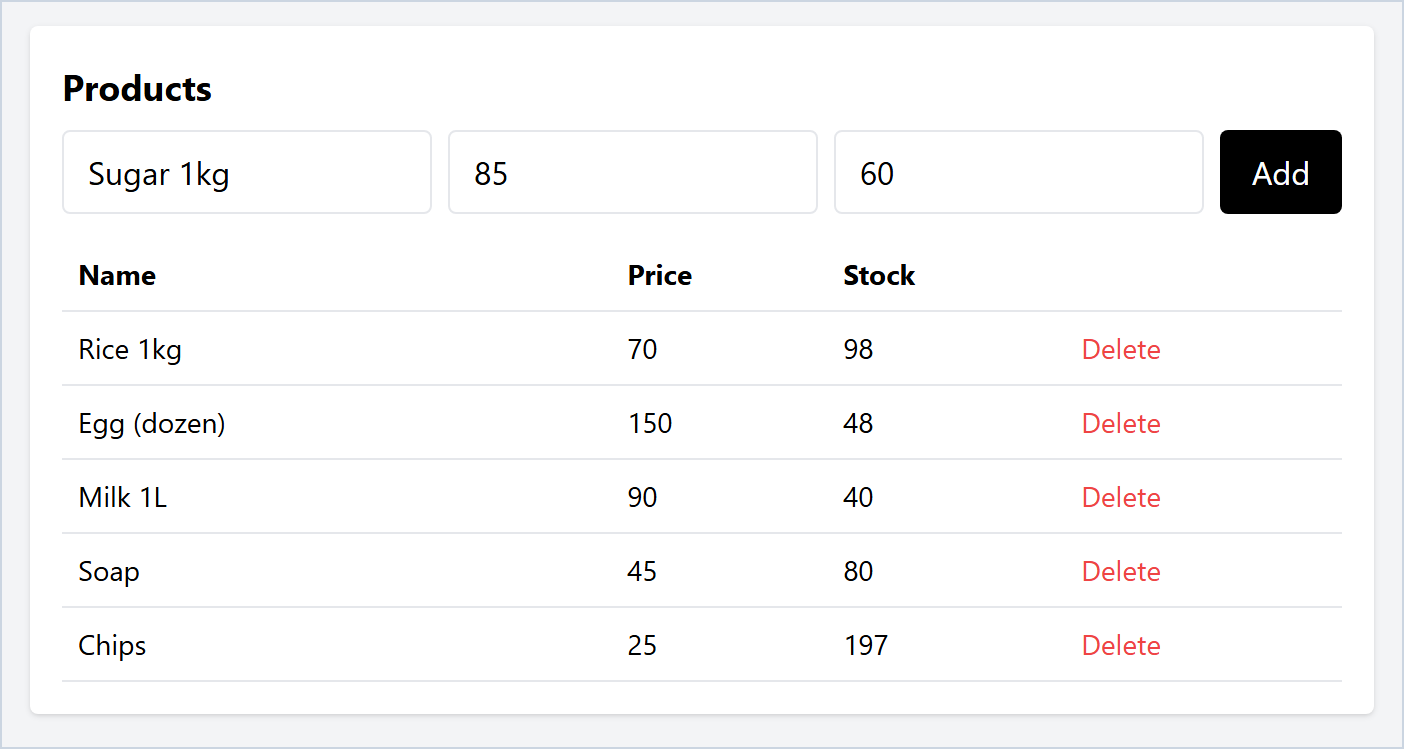
\includegraphics[width=0.62\textwidth]{../screenshots/04_products.png}
\caption{US-4 input side --- the product catalogue with the add-product form used to maintain
price and stock.}
\label{fig:shot-products}
\end{figure}

\begin{figure}[H]
\centering
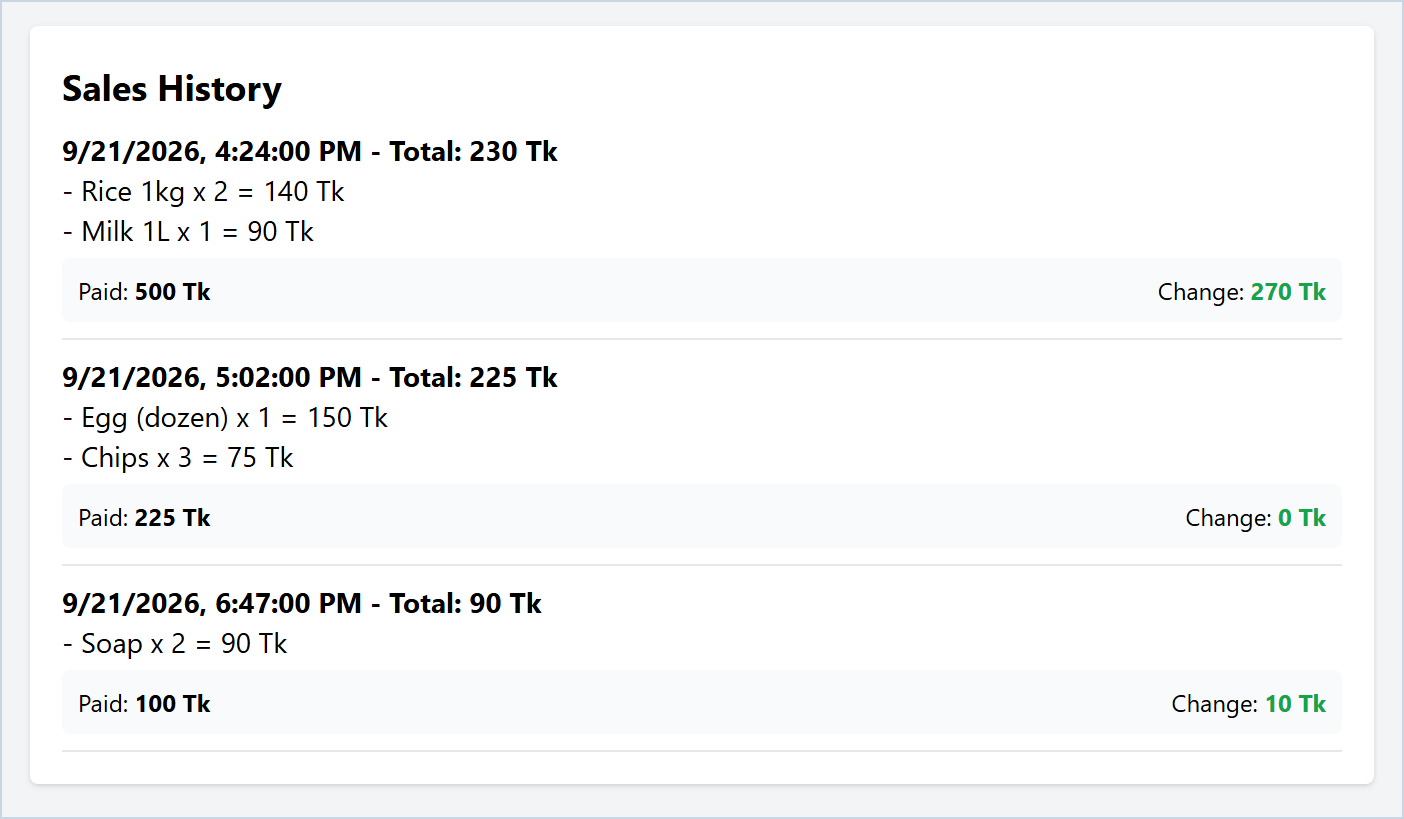
\includegraphics[width=0.62\textwidth]{../screenshots/05_sales_history.png}
\caption{US-6 --- sales history with each bill's timestamp, itemised lines, total, cash paid
and change returned.}
\label{fig:shot-sales}
\end{figure}

\subsection{Backlog carried to the next increment}
\label{sec:mvp-backlog}

The following items were identified during this lab and are planned as the next increment.
They are listed here so that the boundary of the MVP is explicit.

\begin{table}[H]
\centering\small
%% no zebra striping (colortbl not used)
\begin{tabularx}{\textwidth}{@{}p{0.09\textwidth}Xp{0.22\textwidth}@{}}
\toprule
%% no filled header band (colortbl not used)
\multicolumn{3}{c}{\sffamily\bfseries\color{navy} Backlog for the next increment}\\
\midrule
ID & Item & Origin\\
\hline
B-01 & Sales summary dashboard: aggregated total revenue, today's revenue and number of bills, with the supporting summary endpoint & Increment 2 remainder (PR \#2)\\
B-02 & Product edit screen wired to the existing \code{PUT /api/products/:id} route & FR-06 is currently API-only\\
B-03 & Category selection in the add-product form --- the \code{Product} model and the seed data already carry a \code{category} field, but the form does not collect it & Model/UI mismatch noticed in review\\
B-04 & Low-stock indicator and reorder threshold & Objected to by the shop owner scenario: stock is known but not flagged\\
B-05 & Date-range filter and receipt numbering on the sales history & Recurring shop need for end-of-day reconciliation\\
B-06 & Role separation (owner vs.\ cashier) and hashed credentials & Current single shared account is an MVP simplification\\
B-07 & Extract the change calculation into a pure function and add automated unit tests, including a property test that change $\ge 0$ & Preparation for the testing lab\\
\end{tabularx}
\end{table}

% =====================================================================
\section{GitHub Collaboration Evidence}
% =====================================================================
\label{sec:github}

\subsection{Repository}

\begin{center}
\textbf{Repository link:} \repo\\[3pt]
{\small Branches: \filep{main} (integration), \filep{tanzirul/mvp-base},
\filep{ruan/dashboard}, \filep{shuvo/category-receipt},
\filep{tanzirul/report-lab2}}\\[3pt]
{\small Repository contributors (GitHub): \code{TanzirulIslam22},
\code{mahdi-ruan}, \code{Hi-There-shuvo}}
\end{center}

\subsection{Repository directory structure}

\begin{lstlisting}[title={Repository layout}]
QuickPOS/
|-- client/                          React + Vite frontend (Increment 1)
|   |-- src/
|   |   |-- api.js                   base URL + getJSON / postJSON helpers
|   |   |-- App.jsx                  app shell, session gate, page navigation
|   |   |-- main.jsx                 React entry point
|   |   |-- index.css                Tailwind entry point
|   |   `-- pages/
|   |       |-- Login.jsx            staff login screen
|   |       |-- Products.jsx         product catalogue (list / add / delete)
|   |       |-- POS.jsx              billing: cart, total, cash, checkout
|   |       |-- Sales.jsx            sales history
|   |       `-- Invoice.jsx          printable receipt modal   (Increment 3)
|   |-- index.html                   Vite entry template
|   |-- vite.config.js               dev server + build config
|   |-- tailwind.config.js           Tailwind content paths
|   |-- postcss.config.js            PostCSS pipeline
|   `-- package.json
|-- server/                          Express + MongoDB backend (Increment 1)
|   |-- server.js                    app bootstrap, DB connect, /api/seed
|   |-- models/
|   |   |-- Product.js               name, price, stock, category
|   |   `-- Sale.js                  items, total, paidAmount, change, date
|   |-- routes/
|   |   |-- productRoutes.js         GET/POST/PUT/DELETE /api/products
|   |   `-- saleRoutes.js            GET/POST /api/sales   (NFR-10 check)
|   |-- .env.example                 documented configuration template
|   `-- package.json
|-- docs/
|   |-- Project_Design_Report.tex    LaTeX source of this report
|   |-- Requirement_Report.pdf       this report (compiled)
|   `-- TEAM_WORKFLOW.md             branching, PR and review rules
|-- assets/                          design assets used by the report
|-- screenshots/                     MVP screen captures (Section 8.8)
|-- lab_2.pdf                        lab manual
`-- README.md                        project overview, API table, team
\end{lstlisting}

\begin{notebox}[Note on the suggested \filep{src/} folder]
The lab manual's suggested layout lists a single \filep{src/} directory. QuickPOS keeps its
source in two top-level modules, \filep{client/src} (frontend) and \filep{server} (backend),
so that the two separately buildable and separately deployable layers stay separated. This
is the same separation the manual asks for, expressed at the deployment boundary rather than
inside one folder.
\end{notebox}

\subsection{Branching strategy}

\begin{table}[H]
\centering\small
%% no zebra striping (colortbl not used)
\begin{tabularx}{\textwidth}{@{}p{0.26\textwidth}p{0.19\textwidth}X@{}}
\toprule
%% no filled header band (colortbl not used)
\multicolumn{3}{c}{\sffamily\bfseries\color{navy} Branching strategy}\\
\midrule
Branch & Owner & Purpose\\
\hline
\filep{main} & All (integration only) & Stable, reviewed, integrated codebase; the only branch that is deployed or demonstrated\\
\filep{tanzirul/mvp-base} & Tanzirul Islam & Increment 1 --- POS core baseline\\
\filep{ruan/dashboard} & Ruan & Increment 2 --- sales summary (partially delivered)\\
\filep{shuvo/category-receipt} & Shuvo & Increment 3 --- printable invoice / receipt\\
\filep{tanzirul/report-lab2} & Tanzirul Islam & Increment 4 --- report, workflow documentation and screenshots\\
\end{tabularx}
\end{table}

\subsection{Pull requests}

\begin{table}[H]
\centering\small
\setlength{\tabcolsep}{4pt}
%% no zebra striping (colortbl not used)
\begin{tabularx}{\textwidth}{@{}p{0.055\textwidth}p{0.185\textwidth}p{0.325\textwidth}p{0.135\textwidth}p{0.21\textwidth}@{}}
\toprule
%% no filled header band (colortbl not used)
\multicolumn{5}{c}{\sffamily\bfseries\color{navy} Table: Pull requests raised against \filep{main}}\\
\midrule
PR & Head branch & Title & Diff & State / outcome\\
\hline
\#1 & \filep{tanzirul/mvp-base} & \code{docs: add QuickPOS team}\newline\code{information} & $+28/-15$\newline 1 file & Open --- superseded by PR \#4, which carries the final documentation set\\
\#2 & \filep{ruan/dashboard} & \code{feature: add sales summary}\newline\code{and endpoint and}\newline\code{dashboard page} & $+1/-5$\newline 2 files & Merged 21 Sep 2026 --- partial (see Section~\ref{sec:increment2})\\
\#3 & \filep{shuvo/category-receipt} & \code{Feature - Invoice function}\newline\code{added} & $+204/-45$\newline 2 files & Merged 21 Sep 2026 --- complete\\
\#4 & \filep{tanzirul/report-lab2} & \code{Increment 4: project design}\newline\code{report, workflow docs}\newline\code{and MVP screenshots} & docs set & Merged into \filep{main} --- complete\\
\end{tabularx}
\end{table}

\subsection{Commit history}

The history below is the actual output of \code{git log --graph} on \filep{main}. The merge
commits make each increment visible as a separate, reviewable unit, and the author line of
each non-merge commit identifies the member who wrote it.

\begin{lstlisting}[title={git log --graph main}]
*   2cbd99a  Merge pull request #3 from TanzirulIslam22/shuvo/category-receipt
|\
| * da55ea0  Feature - Invoice function added            (Hi-There-shuvo)
|/
*   ce4f8a1  Merge pull request #2 from TanzirulIslam22/ruan/dashboard
|\
| * a0f9b10  feature: add sales summary and endpoint     (mahdi-ruan)
| |          and dashboard page
|/
*   64d8f4d  feat: initial QuickPOS MVP (login,          (TanzirulIslam22)
|           products, billing, sales, cash handler)
\end{lstlisting}

\begin{lstlisting}[title={Contribution by branch (git log --format, per branch}]
tanzirul/mvp-base      64d8f4d  Tanzirul Islam  initial MVP baseline
ruan/dashboard         a0f9b10  Ruan            sales summary increment (partial)
shuvo/category-receipt da55ea0  Shuvo          invoice / receipt increment
\end{lstlisting}

\subsection{Pull request review protocol}

\begin{itemize}
  \item A feature branch is opened from an up-to-date \filep{main}
        (\code{git pull origin main} first), so that branches stay short-lived and conflicts
        are rare.
  \item The pull request description states the increment number, the requirements it
        satisfies, and anything left unfinished.
  \item At least one other team member reviews and approves before the merge; review comments
        are resolved rather than dismissed.
  \item Conflicts are resolved locally by the pull request author, re-tested, and re-pushed
        for a final review pass.
  \item No direct pushes to \filep{main}. Every change lands through a reviewed pull request.
\end{itemize}

\subsection{Collaboration issues encountered}

\begin{itemize}
  \item \textbf{Branch and title drift.} Two branch names promised more than their increments
        delivered (\filep{ruan/dashboard}, \filep{shuvo/category-receipt}). The team resolved
        this by recording the \emph{actual} merged diff per pull request in
        Table~\ref{tab:increments} and by numbering the remaining work as backlog items,
        rather than letting the branch name stand as the description.
  \item \textbf{Local branch drift.} Working from a feature branch that had fallen behind
        \filep{main} left changes staged in the index that no longer matched any branch.
        Resolution: \code{git fetch} and fast-forward \filep{main} to \code{origin/main}
        before starting new work, and never leave unrelated changes staged.
\end{itemize}

% =====================================================================
\section{Challenges Encountered and Engineering Mitigations}
% =====================================================================

\subsection{C-1: The first report build rendered faint, low-contrast text}

The first version of this report was compiled without outline fonts being available, so
pdfTeX fell back to 1-bit bitmap (PK) fonts. The result was text drawn from very low
resolution bitmaps: thin, jagged strokes with poor contrast that were difficult to read on
screen and poor in print.

\textbf{Mitigation.} The document now loads an explicit Type 1 outline family (Latin Modern
for body text, Helvetica for headings) and applies a fixed, deliberately dark colour scheme:
body text is near-black rather than grey, headings use a dark navy and a dark teal, and
table rules and text stay dark. The build was verified afterwards by inspecting the font
objects embedded in the output PDF and confirming that they are Type 1 outlines with no
Type 3 bitmap fonts present. This is the change requested after reviewing the earlier draft.

\subsection{C-2: Client-side payment validation is not enforcement}

An early concern was that a sale could be recorded with insufficient cash, since the cash
amount is entered in the browser.

\textbf{Mitigation.} Validation is deliberately duplicated. The client disables the
\emph{Checkout} button and marks the amount as insufficient, which is a usability measure;
the server independently recomputes the total, rejects \code{paidAmount $<$ total} with HTTP
400 \emph{before} writing anything, and is the only component whose check counts (NFR-10).

\subsection{C-3: A sale could have partially decremented stock}

Validating each cart line while decrementing it would leave stock corrupted if a later line
failed --- for example, if a customer asked for 3 of an item that only had 1.

\textbf{Mitigation.} The route first builds the full list of bill items, validating stock for
every line, and only then performs the writes; a rejected sale therefore leaves stock exactly
as it was (NFR-12, FR-14). The requirement is captured as a user story with an explicit
acceptance criterion (US-4).

\subsection{C-4: An increment was merged with less delivered than its branch name promised}

Pull request \#2 was named and titled as a dashboard increment but merged only route-level
changes, leaving the actual summary widget undelivered.

\textbf{Mitigation.} Three changes followed. First, the report states the delivered scope of
each increment from the merged diff rather than from the branch name
(Section~\ref{tab:increments}). Second, the remainder is recorded as backlog item B-01 with a
named owner. Third, the team's review protocol now requires every pull request description to
declare unfinished work explicitly, so an incomplete increment is visible in the repository
itself and not only in a report.

\subsection{C-5: Environment differences between machines}

Each member develops on a different machine, and the database connection string differs
between them.

\textbf{Mitigation.} A documented \filep{server/.env.example} is committed, the real
\filep{.env} is listed in \filep{.gitignore} so no connection string can be committed by
accident, and the port is read from the environment with a default, so a member's local port
choice cannot break the frontend contract.

\subsection{C-6: The billing component was growing beyond a single responsibility}

Adding the receipt to the billing screen pushed \filep{POS.jsx} towards handling cart
state, payment validation and receipt rendering in one place.

\textbf{Mitigation.} The receipt was extracted into its own \filep{Invoice.jsx} component
that receives the completed sale and a close callback as its only interface. POS keeps
ownership of the cart and payment flow, the invoice owns presentation and printing, and the
print stylesheet is scoped to the modal via an \code{@media print} block and a
\code{no-print} utility class (NFR-15).

% =====================================================================
\section{Conclusion}
% =====================================================================

In Lab 2 the team analysed a real retail problem, documented eighteen functional and fifteen
non-functional requirements with traceability to the delivered code, selected and justified
the Incremental Development process model, and delivered a working MVP of a super shop POS
system: authenticated billing, a maintained product catalogue, cart and total computation,
cash handling with change calculation, automatic stock validation and deduction, a printable
invoice, and a persistent sales history --- built with React, Vite, Tailwind CSS, Express and
MongoDB.

The Incremental model proved practical rather than merely formal. Four increments were
planned and delivered as four reviewable units on four feature branches, and the model made
the one incomplete increment visible: instead of Increment 2 disappearing into a vague commit
message, its remainder is a named backlog item with an owner. Collaboration followed the same
shape --- no direct pushes to the integration branch, every change landed through a reviewed
pull request, and each member's contribution is traceable in the commit history and in the
ownership tables of this report.

As the first milestone of a semester-long project, QuickPOS was deliberately built as small,
replaceable modules with a single API client module and a single route layer, so that the
design-pattern and testing labs can add to the system incrementally rather than requiring a
rewrite. The immediate next increment is defined in Section~\ref{sec:mvp-backlog}: the sales
summary dashboard, the product edit screen, category selection, a low-stock indicator,
date-range reporting, role separation, and unit tests for the cash-handling arithmetic.

% =====================================================================
\begin{thebibliography}{9}
\small
\bibitem{rubric} Department of Computer Science \& Engineering, RUET.
  \emph{CSE 3206 --- Software Engineering Sessional, Lab 2: Software Process Models,
  Requirement Analysis \& MVP Development} --- lab manual and assessment rubric.

\bibitem{pressman} Pressman, R. S. and Maxim, B. R.
  \emph{Software Engineering: A Practitioner's Approach}. McGraw-Hill.
  (Source of the process-model definitions used in Sections~\ref{sec:model}
  and~\ref{sec:justification}.)
\end{thebibliography}

\end{document}
